\documentclass[10pt]{scrartcl}
\usepackage{graphicx}
\usepackage[default]{opensans}
\usepackage{sfmath} % sans font also for math
 \usepackage[binary-units = true]{siunitx}

% defining the paper layout that no text overlaps with the header
\usepackage[
  top=35mm,
  headheight=25mm,
  headsep=3mm,
  bottom=30mm,
  left=25mm,
  right=25mm
]{geometry}

\usepackage{latexsym}
\usepackage[centertags]{amsmath}
\usepackage{amssymb}

% custom header and footpage
\usepackage{scrpage2}
\pagestyle{scrheadings} % you have to set the custom layout
\ihead{} % left head
\ohead{
\includegraphics[height=25mm]{EUCALL.png}}
\ifoot{
\includegraphics[height=13.4mm]{EU.png}} % left foot
\cfoot{
  \begin{minipage}{100mm}
    \begin{scriptsize}
      \normalfont{This project has received funding from the}
      \textit{European Union’s Horizon 2020 research and innovation programme}
      \normalfont{under grant agreement No 654220.}
    \end{scriptsize}
  \end{minipage}
} % center foot
\ofoot{\thepage} % right foot
\chead{}

\usepackage{booktabs} % more eye candy for tables

% sophisticated linking of references in the pdf and setting some options
\usepackage{url}                                                  % for correct typesettings of URLs
\usepackage{hyperref}                                             % for sophisticated linking of urls, dois, pictures, tables, etc.
\hypersetup{
    unicode=true,                                                 % non-Latin characters in Acrobat’s bookmarks
    pdftoolbar=true,                                              % show Acrobat’s toolbar?
    pdfmenubar=true,                                              % show Acrobat’s menu?
    pdffitwindow=false,                                           % window fit to page when opened
    pdfstartview={FitH},                                          % fits the width of the page to the window
    pdftitle={D4.1: Short pulse laser-matter interaction simulations},                                        % title
    pdfauthor={C. Fortmann-Grote},                                           % author
    pdfsubject={EUCALL WP4 (SIMEX) deliverable 4.1},                             % subject of the document
    pdfcreator={pdflatex},                                         % creator of the document
    pdfkeywords={EUCALL, SIMEX, simulations, PIC, XFEL, scattering},                                         % list of keywords
    pdfnewwindow=true,                                            % links in new PDF window
    colorlinks=true,                                              % false: boxed links; true: colored links
    linkcolor=blue,                                                % color of internal links (change box color with linkbordercolor)
    citecolor=blue,                                                % color of links to bibliography
    filecolor=blue,                                               % color of file links
    urlcolor=blue                                                 % color of external links
}

% Zeilenabstand
\renewcommand{\baselinestretch}{1.2}


%\renewcommand*\chapterpagestyle{scrheadings} % otherwise chapter start is plain ;-); works only for KOMA script; plain LaTeX works different

%%%%%%%%%%%%%%%%%%%%%%%%%%%%%%%%%%%%%%%%%%%%%%%
%   BIBLIOGRAPHY SETTINGS                     %
%%%%%%%%%%%%%%%%%%%%%%%%%%%%%%%%%%%%%%%%%%%%%%%
\usepackage[bibstyle=nature,sorting=none,=maxnames=1000,eprint=false,
defernumbers=true, backend=biber]{biblatex}
\usepackage{hyperref}

\renewcommand*\finalnamedelim{, and\addspace}
\DeclareNameAlias{sortname}{last-first}
\renewcommand{\newunitpunct}{, }

\AtEveryBibitem{%
  \clearfield{day}%
  \clearfield{month}%
  \clearfield{endday}%
  \clearfield{endmonth}%
  \clearfield{issn}%
  \clearfield{issue}%
}
%convert titles to hyperlinks using doi
\ExecuteBibliographyOptions{doi=false} \newbibmacro{string+doi}[1]{%
  \iffieldundef{doi}{#1}{\href{http://dx.doi.org/\thefield{doi}}{#1}}}
  \DeclareFieldFormat*{title}{\usebibmacro{string+doi}{\mkbibemph{#1}}}

\addbibresource{/home/grotec/Documents/LiteratureDB/bibtex/jabref.bib}
%\addbibresource{references.bib}
%%%%%%%%%%%%%%%%%%%%%%%%%%%%%%%%%%%%%%%%%%%%%%%
% END BIBLIOGRAPHY SETTINGS                   %
%%%%%%%%%%%%%%%%%%%%%%%%%%%%%%%%%%%%%%%%%%%%%%%

\begin{document}
\makeatletter
\begin{titlepage}
\thispagestyle{scrheadings}
\begin{center}
$~$\\
\vspace{0cm}
{\Large\textbf{EUCALL}\\[2ex]
The European Cluster of Advanced Laser Light Sources}\\[4ex]
%
{\small\textbf{Grant Agreement number: 654220}}\\[8ex]
%
Work Package 4 -- SIMEX\\[4ex]
%
Deliverable D4.1\\
%
Design Report and Advanced Simulation Software -- Short Pulses
Interaction\\[5ex]
%
Lead Beneficiary: European XFEL\\[5ex]
%
Carsten Fortmann-Grote, Alexander Andreev, Richard Briggs, Michael Bussmann,
  Axel Huebl,\\ Thomas Kluge,
  Sakura Pascarelli, Ashutosh Sharma, and Adrian P. Mancuso\\[4ex]
%
Due data: 30 September 2016\\
Date of delivery: \today \\[4ex]
%
Project webpage: \url{www.eucall.eu}\\[6ex]
%
{%
\small
\begin{tabular}{|l|l|}
  \hline
  \multicolumn{2}{|l|}{ \textit{Deliverable Type} } \\
  \hline
  R = Report\hfill & R \\
  DEM = Demonstrator, pilot, prototype, plan designs & \\
  DEC = Websites, patents filing, press \& media actions, videos, etc. & \\
  OTHER = Software, technical diagram, etc. & \\
  \hline
  \multicolumn{2}{|l|}{\textit{Dissemination level}} \\
  \hline
  PU = Public, fully open, e.g. web & PU \\
  CO = Confidential, restricted under conditions set out in Model Grant
  Agreement\hspace*{17ex}\  & \\
  CI = Classified, information as referred to in Commission Decision 2001/844/EC
  & \\
  \hline
\end{tabular}
}

\end{center}
%
\vfill

\includegraphics[width=\textwidth]{./PartnerLogos.pdf}
\normalfont
\end{titlepage}
\makeatother

\tableofcontents
\begin{abstract}
  \noindent%
  \textbf{Abstract} -- We present a design for integrated simulations of an x-ray scattering
  experiment probing high power femtosecond laser pulses interacting with solid
  matter by small-angle x-ray scattering.
  Coherent x-ray pulses as delivered by an x-ray free-electron laser
  and their propagation through beamline optics are simulated with the
  simulation framework \texttt{simex\_platform}. High power femtosecond optical
  laser pulses interacting with a solid density target are simulated with
  a particle-in-cell code. We trace x-ray photons scattering from the laser excited
  plasma using a MonteCarlo simulation and synthesize a scattering image.
  We present the involved simulation codes and their interfaces.
  An experiment to be simulated is outlined taking into account parameters of optical lasers and
  x-ray pulse properties available at the European X-Ray Free-Electron Laser.
\end{abstract}
%
\section{Introduction}
Ultra-short pulsed high power lasers (HPLs) typically deliver laser
pulses in the infrared (800~nm to 1000~nm) at pulse durations below one
picosecond. Today's high power lasers \cite{Siebold2008} can reach intensities of
up to $10^{21}~\text{W}/\text{cm}^2$ on spot sizes of a few microns and pulse
durations on the order of a few tens of femtoseconds.

Despite their intensity, these sources usually do not penetrate a solid density
target but rather create a plasma at the target front side, accelerating
electrons to relativistic energies in the strong electric field of the
laser~\cite{Kluge2011} and pushing them into the target via the
$\vec{v}\times\vec{B}$ force once the velocity $v$ approaches the speed of
light~\cite{Mulser2010,Gibbon1996}.

The generation of relativistic electrons at the front side, the transport of
electrons through the target and the subsequent formation of a sheath of
electrons at the target rear side all happen on time scales below a few hundred
femtoseconds~\cite{Macchi2013}. They can create plasma
instabilities~\cite{Metzkes2014}, ionize and heat the target
bulk~\cite{Huang2013}, generate strong magnetic fields or drive shocks inside
the target.

These phenomena can potentially be studied with high spatial resolution of a few
nanometers and temporal resolutions of a few femtoseconds using x-ray
lasers~\cite{Kluge2014,Kluge2016} such as the European X-Ray Free Electron
Laser (XFEL).

The particle-in-cell (PIC) method~\cite{Birdsall2004} is an advanced simulation
method to study the interaction of a HPL with a solid density
target. Realistic 3D PIC simulations of laser-irradiated solid
density plasmas require Petascale computing capabilities and produce hundreds of
Terabytes of data~\cite{ornl_picongpu}.

Within the SIMEX workpackage of EUCALL we interface particle-in-cell (PIC) codes
such as \texttt{PIConGPU}~\cite{Bussmann2013, picongpu_github} that describe the solid density plasma to codes that
model the generation and propagation of XFEL pulses to
generate synthetic scattering signals from free and, in the future, bound
electrons. The interfaces, which are based on the openPMD~\cite{openPMD} meta data format, are
part of the software suite \texttt{simex\_platform} \cite{simex_github},
developed in a collaborative effort within SIMEX. A detailed description of
\texttt{simex\_platform} is given in the documentation available via the
software repository \cite{simex_github} and in the technical
milestone M4.1.

As a first test of the simulation capabilities of \texttt{simex\_platform}
free electron density data from a PIConGPU simulation of the interaction of a
short-pulse laser system\footnote{see details below} available at the High
Energy Density (HED) instrument \cite{Nakatsutsumi2014} at the European XFEL
will be used to compute a synthetic scattering signal in a Small-Angle X-ray
Scattering (SAXS) geometry.
%
%\section{Propagation\label{sec:short_pulse_prop}} Propagation of XFEL pulses is
%modeled through the existing XFELPhotonPropagator calculator. The latter is an
%interface to \texttt{WPG} \cite{Samoylova2016, wpg_github}, a python high level
%interface for the \texttt{Synchrotron Radiation Workshop} (SRW)
%\cite{Chubar2008, srw_github}.  The simulation parameters reflect the
%conditions at the High Energy Density (HED) instrument \cite{Nakatsutsumi2014}
%at the European XFEL. The focal spotsize can be fixed at three different
%ranges, $\approx 200 \mu\text{m}$, $\approx 20 \mu\text{m}$, and $\approx 2
%\mu\text{m}$ \marginpar{Fix numbers, how large are the ranges?}
%%
\section{Photon-Matter interaction}
\subsection{Optical Laser}
The short-pulse
optical laser-plasma interaction is modeled with \texttt{PIConGPU}
\cite{Bussmann2013}.

\texttt{PIConGPU} is an Open Source~\cite{picongpu_github} explicit,
relativistic 3D3V\footnote{3D3V denotes the 6 dimensional phase space spanned by 3 position
vector components and three velocity vector components} particle-in-cell (\texttt{PIC}) code which can simulate the
interaction of high power, ultra-short laser pulses with matter.  The
simulations will assume realistic parameters for the optical laser system at the
HED instrument at European XFEL. The most important parameters are summarized in
Table~\ref{tab:short_pulse_laser_parameters}.

\begin{table}[h!]
\centering
\begin{tabular}{l|l}
  \hline
  \hline
  wavelength & 800 nm \\
  pulse duration (fwhm) & 15 fs - 80 fs \\
  focus size (fwhm)  & 3 $\mu\text{m}$ \\
  temporal profile &  Gaussian \\
  spatial profile &  Gaussian \\
  pulse energy & 2 mJ \\
  prepulse contrast & $\approx 10^{-4}$ (energy)\\
  intensity  & $10^{17}$ W/cm$^2$ \\
  \hline
  \hline
\end{tabular}
\caption{European XFEL HED pump-probe laser parameters for optical laser-matter interaction
simulations}
\label{tab:short_pulse_laser_parameters}
\end{table}

HPL pulses are defined by their time dependent
magnetic and electric field components. Their evolution is governed by the
Maxwell equations \cite{Jackson1975}. A PIC code solves these partial differential
equations on a regular mesh (usually
Cartesian) using e.g. finite difference time domain techniques~\cite{Yee1966}.

\subsection{X-ray Laser (Scattering)}

In principle, all imaging techniques employed for probing the interaction
of \texttt{HPL} lasers with targets can be used in the case of ultra-short
pulse lasers as well. However, some of these techniques are limited to slowly
varying plasma conditions (in comparison to the ultra-short laser pulse duration)
and thus are not suitable to capture fast, transient processes. Moreover, atomic
processes, multiple scattering, velocity-dependent scattering and
non-equilibrium plasma conditions cannot always be taken into account with
existing modeling techniques, especially if the x-ray laser pulse itself interacts
with the plasma.

Thus, for ultra-short laser pulses x-ray interaction will in addition to existing
techniques be modeled via a Monte-Carlo photon interaction model. Each photon is
described by its wave vector and a phase\footnote{In the future, the photon model
will also include polarization.}.

The x-ray pulse is described by temporally and spatially varying electric fields
(amplitude, polarization, and phase). At discrete points in time, the field
distribution in a plane perpendicular to the laser axis is converted into a
photon distribution using a conversion tool contained in
\texttt{simex\_platform}. These photons are then tracked through the volume simulated by
\texttt{PIConGPU} using the software \texttt{parataxis}.
Table~\ref{tab:xfel_sase2} gives an overview over the expected x-ray pulse
parameters at the HED instrument at the European XFEL.

\begin{table}[h]
  \centering
  \begin{tabular}{l|l}
    \hline
    \hline
    photon energy &  6 keV - 12 keV \\
    pulse duration & $\approx$ 10 fs \\
    focus size (fwhm) & 2 $\mu\text{m}$ - 200 $\mu\text{m}$\\
    rel. bandwidth & 10$^{-3}$ (SASE) - $10^{-5}$ (seeded)\\
    photons/pulse & 10$^{12}$\\
    \hline
    \hline
  \end{tabular}
  \caption{X-ray pulse parameters for the HED instrument at the European XFEL}
  \label{tab:xfel_sase2}
\end{table}

In describing the interaction of coherent x-rays with the laser excited plasma,
we focus on scattering processes, predominantly Thomson scattering from free
electrons. Further atomic processes, e.g. K-shell ionization and resonant
scattering will be considered later when detailed atomic modelling using the
scFLY code \cite{Chung2007} has become part of the simulation capabilities. This is
currently under development.

The scattering signal will be processed to
infer information about the microscopic and macroscopic state of the plasma
during and after the optical laser-plasma interaction.  Photons are scattered
according to predefined scattering functions that depend on the local properties
of the matter irradiated by the HPL. In the most simple case, the local free
electron density is used as an input for calculating the probability for Thomson
scattering from free electrons.

There are several methods that already are or will in the future be implemented for
scattering. We list them below in order of ascending generality (and technical
difficulty). Due to time limitations only some of these methods will be implemented
during the EUCALL project, but will be added to PIConGPU for future inclusion into
\texttt{simex\_platform} .

\begin{enumerate}
  \item 3D Fast Fourier Transform of electron density
    \label{pmi:methods:fft}
  \item Ex-situ scattering using stand-alone
    Monte-Carlo photon scattering \label{pmi:methods:exsituphoton}
  \item In-situ scattering using a modified particle-in-cell algorithm and far field
      Lienard-Wiechert potential calculation \label{pmi:methods:insitulienardwiechert}
    \item In-situ scattering using Monte-Carlo photon
    scattering\label{pmi:methods:insituphoton}
  \item In-situ scattering using Monte-Carlo photon scattering with absorption
    and emission of photons\label{pmi:methods:insituphotoninteract}
\end{enumerate}

Ex-situ Fast Fourier Transforms have been implemented using the \texttt{LiFFT}
library \cite{liblifft_github} and can be performed in a post processing step on
\texttt{openPMD} outputs of the electron density. Implementation in
\texttt{simex\_platform} is currently under discussion.

Ex-situ scattering is performed by the \texttt{paraTAXIS} code.
The code is still in closed source development and is planned to be released as open
source within the EUCALL funding period.
It uses the same libraries and
techniques as \texttt{PIConGPU}. Specifically, it can read
\texttt{openPMD}~\cite{openPMD} files via
\texttt{libSplash}~\cite{libSplash_github} and traces photons through a mesh
using \texttt{libPMacc}~\cite{picongpu_github}. One can define an arbitrary
interaction using a C++ function object. The current code version provides
Thomson Scattering from free electrons based on the local electron density.
Photon scattering is computed via repeated Monte-Carlo evaluation of the
scattering function, allowing for multiple scattering.

In-situ scattering using Lienard-Wiechert potentials will be based on an already
existing in-situ Lienard-Wiechert potential calculator plugin to
\texttt{PIConGPU} \cite{Pausch2013}. This method will serve mainly as a cross
check to the other methods. It involves a modification of the PIC algorithm that
will be implemented in the future. The method allows to compute arbitrary
angular far field scattering spectra during the interaction of the HPL with
matter.

An implementation of in-situ Monte-Carlo photon scattering in \texttt{PIConGPU}
would be based on the techniques developed for the \texttt{paraTAXIS} code. Here, the
main issue is the large memory consumption by the photons traced while the
simulation is running.

In addition to elastic scattering of photons from electrons,
excitation of ions, absorption and emission of photons via bound-bound
transitions,
bound-free transitions (photo-ionization, Auger decay, shake-off processes, recombination),
and free-free transitions (bremsstrahlung) will be considered in
the future. The latter are incoherent processes contributing to the background
radiation and their consideration is hence an important step towards a more
realistic simulation of the scattering signal.

In summary, the outlined
framework of physical models will in the future enable fully kinetic in-situ radiation
transport modeling in a particle-in-cell code.
As discussed, development of these capabilities is ongoing and completed tools
will be made available in \texttt{simex\_platform} and \texttt{PIConGPU}.
Compatibility of all software packages will be ensured by reuse of existing
libraries and the common meta data format \texttt{openPMD}.

\section{Simulation workflow}
%
\begin{figure}[ht]
  \begin{center}
    \includegraphics[height=\textwidth, angle=90,clip]{xfel-pic_schema}
  \end{center}
  \caption{Block diagram for integrated simulations of x-ray scattering from a high
  power laser excited plasma.}
  \label{fig:xfel-pic_schema}
\end{figure}

The simulation workflow is depicted in Fig.~\ref{fig:xfel-pic_schema}. The x-ray
pulse generation and propagation is modeled in \texttt{simex\_platform} with the
corresponding simulation codes. The simulated wavefronts are evaluated at the
target surface and converted into a photon distribution. The photons are then
propagated through the target. At discrete timesteps, each photon's wavevector
undergoes a change in magnitude and direction with a
certain probability, given by the Thomson scattering cross section
\cite{Jackson1975}. In this way, multiple scattering events that become
important especially in compressed regions of the target, are naturally
included. Finally, the photon wavefunction is collapsed onto the detector plane
and integrated over the exposure time to obtain the simulated scattering image.
%
%
\section{Experimental scenario}
%
\begin{figure}[ht]
  \begin{center}
    \includegraphics[width=1.0\textwidth,angle=0,clip, viewport=0 30 700 480]{bussmann_saxs_setup}
  \end{center}
  \caption{Schematic rendering of the proposed experiment to be simulated.
  Ultra-short pulsed optical laser radiation (red beam) creates a plasma layer on
a metal foil's surface and accelerates electrons and ions. The XFEL beam (blue)
probes the plasma perpendicular to the optical laser axis. A pixel area detector
captures photons scattered in forward direction.}
  \label{fig:xfel-saxs_setup}
\end{figure}
%
\begin{figure}[ht]
  \begin{center}
    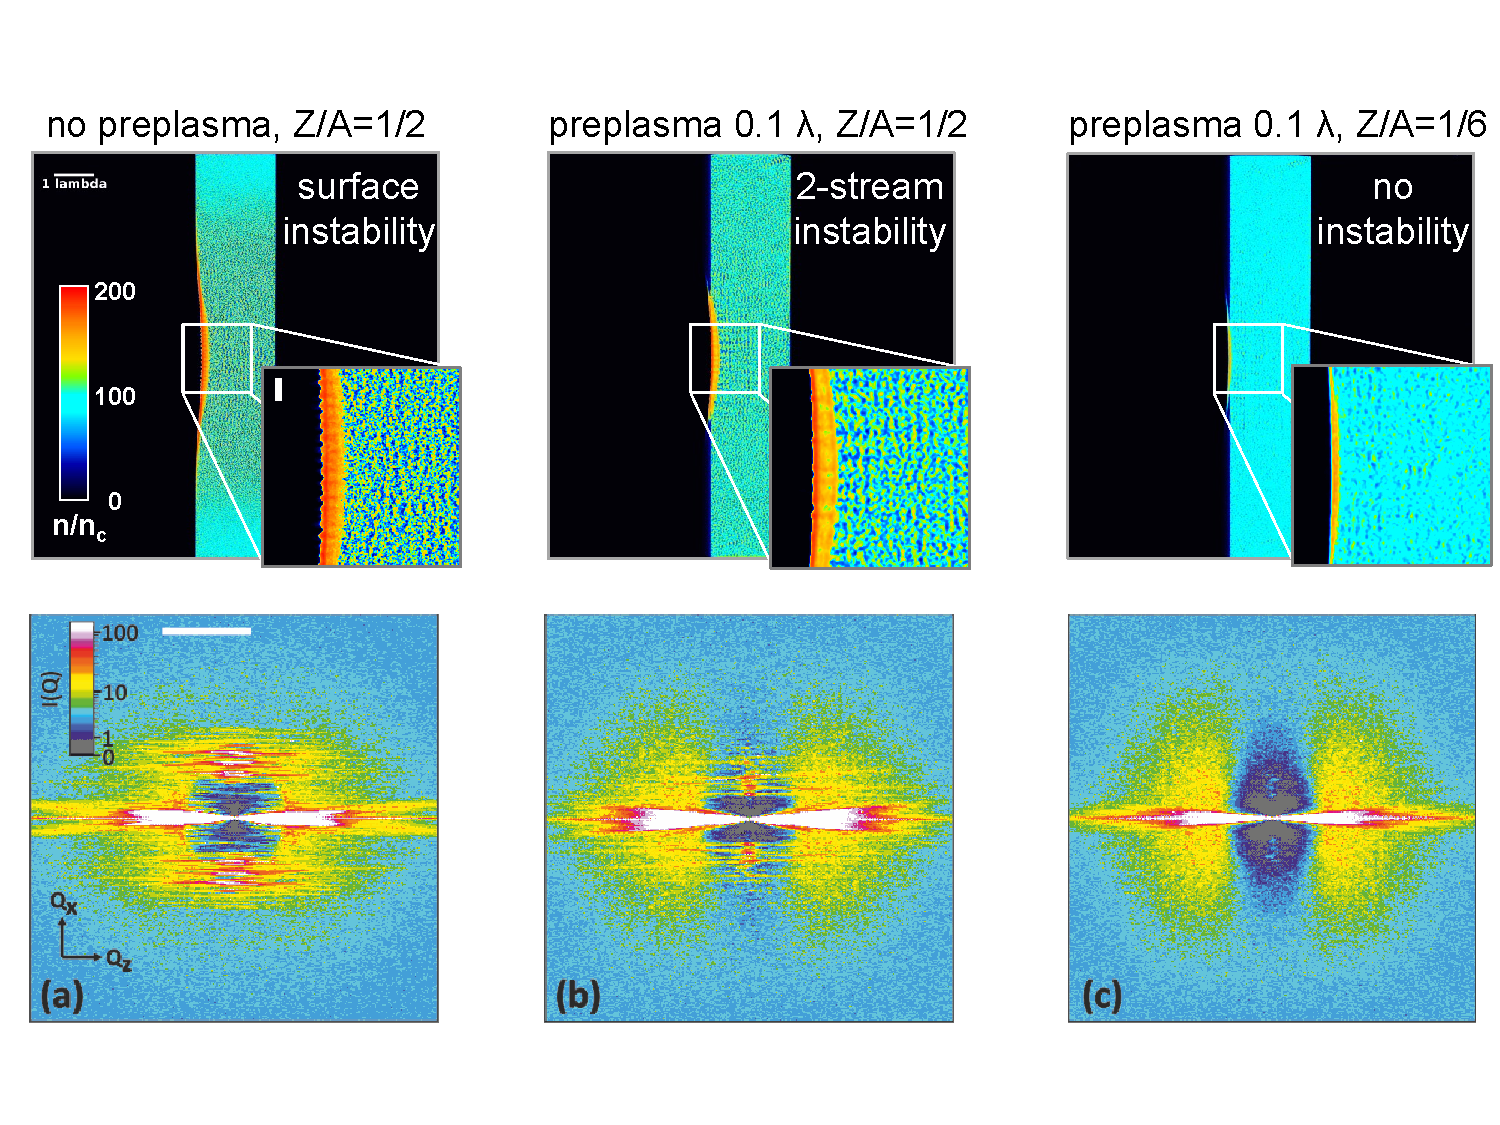
\includegraphics[width=1\textwidth,angle=0,clip]{bussmann_saxs_instabilities}
  \end{center}
  \caption{PIC simulations of the electron density (top) and forward scattering
    patterns (bottom) for various
  types of laser-plasma instabilities.}
  \label{fig:saxs_instabilities}
\end{figure}

We briefly outline an experiment that we plan to simulate with
the tools described above. The experiment would be carried out at the HED
instrument at the European XFEL. We propose a SAXS setup, illustrated in
Fig.~\ref{fig:xfel-saxs_setup}, where a thin metal foil is
first excited using the short pulse HED PP laser and subsequently probed by XFEL
photons.
The choice of the target material depends on the precise x-ray photon energy.
The target material's K-shell absorption edge should be located slightly
below the probe's wavelength to limit x-ray absorption. In resonant
SAXS, the target material's K-shell transitions must match the x-ray photon
energy. Assuming a photon energy of 8 keV, copper is a suitable target material
for normal SAXS and resonant SAXS.

The HED PP laser will
create a plasma of a few to ten micrometer size in the transverse dimension with
respect to the XFEL beam. Hence, we choose 10 micrometer for the focal spot size
to irradiate the full plasma length. A relative bandwidth of
$\approx 10^{-3}$ in SASE mode, corresponding to a few eV in absolute energy is
suitable for a resonant SAXS experiment to ensure efficient excitation of all
involved transitions. This bandwidth is also adequate for non-resonant SAXS.

Through observation of distinct features in the
scattering signal being signatures of resonant modes and instabilities in the
plasma, we will extract information about these modes such as their amplitude
and growth rate under varying experimental conditions such as laser power,
incidence and probe angles. Fig.~\ref{fig:saxs_instabilities} shows three
simulated scattering patterns emerging from interaction of coherent x-rays with
different types of plasma instabilities~\cite{Kluge2014}.
It should be noted that these simulations make idealistic assumptions about the
properties of the x-ray probe. An important aspect of this work is the question
if the observed characteristics will remain so clearly distinct if realistic
simulated pulses are employed in the scattering simulation. Comparison to experimental
data will serve as a validation check of the simulation chain.

\section{Synergy aspects}

The main synergetic aspect of this work is that it allows scientists interested
in short-pulse laser matter interaction to simulate their work under realistic
conditions regarding the physical properties of x-ray pulses, beamline optics,
and x-ray detectors.
In bringing together knowledge and expertise from the high-power
laser-matter interaction community, x-ray optics, and small angle x-ray
scattering, we create unique opportunities for exploring the parameters
at which to best perform the outlined experiment and others of similar character.

As a synergetic byproduct of the simulations outlined above, a
novel application for \texttt{simex\_platform} has emerged,
in which we will
study the concept of a laser-plasma based coherent x-ray source. The PIC
simulation yields the distribution of electrons that are accelerated in the
laser direction up to GeV energies due to the strong electric and
magnetic fields of the HPL. This data can be fed into an FEL simulation code
(e.g. \texttt{genesis} \cite{Reiche1999}) to model the process of
self-amplification by stimulated emission (SASE). These simulations would enable
scientists to develop precise and realistic concepts for such a laser based FEL.

%\section{Detection} At an early stage, the detector will be modeled as an ideal
%x-ray detector, i.e. registering the exact number of incident photons in each
%pixel as simulated by the scattering module. At a later stage, the realistic
%detector response will be modeled within the x-ray Camera Simulation Toolkit
%\cite{Joy2015}.% as described in \cite{Rueter2016_submitted}.
%%
%\section{Data analysis} From the small-angle x-ray scattering data one can
%infer important information about the structure of the highly excited target
%during the interaction with the optical laser. E.g. the electron density is
%directly encoded in the diffraction pattern. In order to reconstruct the
%electron density from the diffraction data, the complex phase of the probe has
%to be reconstructed using an iterative phasing algorithm. Such algorithms are
%widely available, e.g. \ldots \marginpar{Fill in}.  The so calculated electron
%density can then be compared to the particle data in the PIC simulation to
%assess the reliability of the phasing algorithm under given realistic
%experimental condition. \marginpar{What else would be of interest here?}
\section{Summary and Outlook}
In this report we have outlined concepts for the simulation of a SAXS
x-ray scattering experiment probing the interaction of solid density matter
(e.g. a metal foil) with ultra-short (femtosecond) high power optical laser
radiation. The simulations describe all parts of the experiment by exploiting
various codes: The generation of coherent x-ray radiation as well as the
propagation from the source to the experiment through collimating and focussing
optics is modelled with the corresponding codes that are already integrated in
\texttt{simex\_platform}. We than utilize a conversion tool that switches from a
classical wavefront representation of the x-ray radiation to a photon picture,
assigning each photon a wavevector and a phase. The photons are than traced
through the laser generated plasma using a MonteCarlo description of scattering
processes. The plasma itself
is simulated with the particle-in-cell code PIConGPU. Photons
escaping the target from the rear side are finally propagated to the detector
plane, where a scattering image is synthesized. These simulations allow to
assess the influence of realistic x-ray pulse properties on the quality of the
scattering signal. We can test if the identification of plasma
instabilities through characteristics of the scattering signal works under real
world scenarios.
The experiment we propose is designed around the expected optical and x-ray
laser parameters.

Future developments will improve the description of x-rays propagating through
the plasma by including more interaction processes for absorption, scattering,
and emission. It is also planned to integrate the involved simulation codes more
tightly into \texttt{simex\_platform}. In addition, a full detector simulation,
including particle generation, charge transport and electronics will be added.

As a novel application for \texttt{simex\_platform}, we plan to simulate a
laser-plasma accelerator based free electron laser by feeding the output of the
PIC simulation, i.e. the phase space distribution of accelerated electrons into
a FEL simulation code to investigate the possibility of laser based FELs with
realistic electron bunch properties.

\printbibliography[]

\end{document}


